\scanpage{8}
\mspage{6}
\margin{\unsure{2}}
\figure{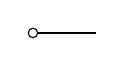
\begin{tikzpicture}[x=1cm,y=1cm]\draw (0,0) circle (.06);\draw (.06,0)--(.8,0);\end{tikzpicture}}

2.2. La sous-extension $\unsure{\bar K_e|\widetilde K_e}$ de $\bar K/K$ est galoisienne, et son groupe de Galois est canoniquement isomorphe au groupe de Galois
\[
(2.2.1)\qquad\pi_0=\operatorname{Gal}(\bar k/k).
\]
On obtient ainsi une suite exacte
\diagram{\begin{tikzcd}[ampersand replacement=\&]
(2.2.2)\quad 1\arrow[r,no head]\&I\arrow[r]\&\pi\arrow[r]\&\pi_0\arrow[r]\&1,
\end{tikzcd}}
où
\[
 I=\operatorname{Gal}(\bar K/\widetilde K)
\]
est ce qu'on appelle le groupe d'\uline{inertie}. \deleted{\unsure{En}} \deleted{\unsure{C'est aussi}} Si on se rappelle que $\widetilde K=$ corps des fractions de $\widetilde V$, \inserted{et que} $\bar K$ est une clôture séparable de $\widetilde K$, on voit donc que $I$ est le groupe de Galois qui correspond à la situation \deleted{\unsure{d'un}} de l'anneau de valuation discrète \uline{strictement local} $\widetilde V$. Si $k$ est sép. clos, on aura $K=\widetilde K$, $V=\widetilde V$, $I=\pi$.

\uline{L'objet du séminaire est} plutôt \uline{l'étude des représentations $\ell$-adiques du groupe d'inertie} $I$. (Ce groupe, ou son image par la représentation $\ell$-adique envisagée, \deleted{\unsure{peut dans le}} est parfois appelé \uline{groupe de monodromie locale}) Il revient au même de dire qu'on s'attachera surtout à étudier les repr. $\ell$-adiques d'un groupe $\pi$, lorsque $k$ est sép. clos. Dans certaines situations cependant, on aura une représentation d'une extension
\margin{7}
